\documentclass{standalone}

\usepackage{tikz}
\usepackage[T1]{fontenc}
\usepackage[tt=false, type1=true]{libertine}
\usepackage[varqu]{zi4}
\usepackage[libertine]{newtxmath}

\usetikzlibrary{shapes, positioning, calc}

\begin{document}

{\scriptsize
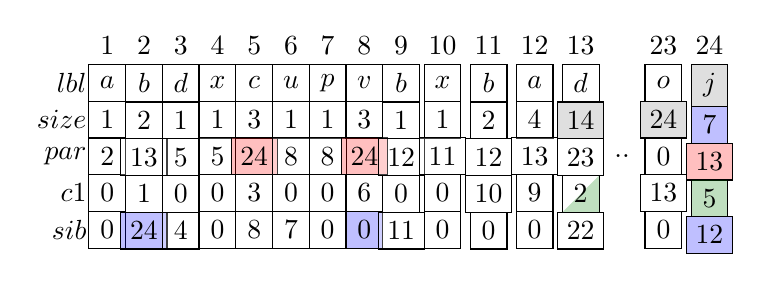
\begin{tikzpicture}
  \newcommand\arraypartspacing{0.015} % 0.03 for thick
  \newcommand\listelemminwidth{0.4675cm }
  \newcommand\listelemminheight{0.4675cm}

  \tikzset{
  diagonal fill/.style 2 args={fill=#2, path picture={
    \fill[#1] (path picture bounding box.south west) -|
              (path picture bounding box.north east) -- cycle;}}}

  \tikzset{generalfill/.style={fill opacity=0.25, text opacity=1}}
  \tikzset{nofill/.style={generalfill, fill=white}}
  \tikzset{redfill/.style={generalfill, fill=red}}
  \tikzset{greenfill/.style={generalfill, fill=black!50!green}}
  \tikzset{bluefill/.style={generalfill, fill=blue}}
  \tikzset{reddiagonalfill/.style={generalfill, diagonal fill={red}{white}}}
  \tikzset{greendiagonalfill/.style={generalfill, diagonal fill={black!50!green}{white}}}
  \tikzset{bluediagonalfill/.style={generalfill, diagonal fill={blue}{white}}}
  \tikzset{grayfill/.style={generalfill, fill=gray}}

  \node[minimum width=\listelemminwidth, minimum height=\listelemminheight] at (0, 0) (ni1) {$1$};
  \node[draw, minimum width=\listelemminwidth, minimum height=\listelemminheight, below=-\arraypartspacing of ni1] (ni1-1) {$a$};
  \node[draw, minimum width=\listelemminwidth, minimum height=\listelemminheight, below=-\arraypartspacing of ni1-1] (ni1-2) {$1$};
  \node[draw, minimum width=\listelemminwidth, minimum height=\listelemminheight, below=-\arraypartspacing of ni1-2] (ni1-3) {$2$};
  \node[draw, minimum width=\listelemminwidth, minimum height=\listelemminheight, below=-\arraypartspacing of ni1-3] (ni1-4) {$0$};
  \node[draw, minimum width=\listelemminwidth, minimum height=\listelemminheight, below=-\arraypartspacing of ni1-4] (ni1-5) {$0$};

  \node[left=-0.1 of ni1-1] {$lbl$};
  \node[left=-0.1 of ni1-2] {$size$};
  \node[left=-0.1 of ni1-3] {$par$};
  \node[left=-0.1 of ni1-4] {$c1$};
  \node[left=-0.1 of ni1-5] {$sib$};

  \foreach \label/\size/\parent/\firstchild/\sibling/\sizecol/\parcol/\nextcol/\childcol [count=\prevpoid from 1, evaluate=\prevpoid as \poid using int(\prevpoid+1)] in {b/2/13/1/24/nofill/nofill/bluefill/nofill, d/1/5/0/4/nofill/nofill/nofill/nofill, x/1/5/0/0/nofill/nofill/nofill/nofill, c/3/24/3/8/nofill/redfill/nofill/nofill, u/1/8/0/7/nofill/nofill/nofill/nofill, p/1/8/0/0/nofill/nofill/nofill/nofill, v/3/24/6/0/nofill/redfill/bluefill/nofill, b/1/12/0/11/nofill/nofill/nofill/nofill, x/1/11/0/0/nofill/nofill/nofill/nofill, b/2/12/10/0/nofill/nofill/nofill/nofill, a/4/13/9/0/nofill/nofill/nofill/nofill, d/14/23/2/22/grayfill/nofill/nofill/greendiagonalfill}{
    \node[minimum width=\listelemminwidth, minimum height=\listelemminheight, right=-\arraypartspacing of ni\prevpoid] (ni\poid) {$\poid$};
    \node[draw, minimum width=\listelemminwidth, minimum height=\listelemminheight, below=-\arraypartspacing of ni\poid] (ni\poid-1) {$\label$};
    \node[draw, minimum width=\listelemminwidth, minimum height=\listelemminheight, below=-\arraypartspacing of ni\poid-1, \sizecol] (ni\poid-2) {$\size$};
    \node[draw, minimum width=\listelemminwidth, minimum height=\listelemminheight, below=-\arraypartspacing of ni\poid-2, \parcol] (ni\poid-3) {$\parent$};
    \node[draw, minimum width=\listelemminwidth, minimum height=\listelemminheight, below=-\arraypartspacing of ni\poid-3, \childcol] (ni\poid-4) {$\firstchild$};
    \node[draw, minimum width=\listelemminwidth, minimum height=\listelemminheight, below=-\arraypartspacing of ni\poid-4, \nextcol] (ni\poid-5) {$\sibling$};
  }

  \node[minimum width=\listelemminwidth, minimum height=\listelemminheight, right=-\arraypartspacing of ni13] (ni14) {};
  \node[minimum width=\listelemminwidth, minimum height=\listelemminheight, below=-\arraypartspacing of ni14] (ni14-1) {};
  \node[minimum width=\listelemminwidth, minimum height=\listelemminheight, below=-\arraypartspacing of ni14-1] (ni14-2) {};
  \node[minimum width=\listelemminwidth, minimum height=\listelemminheight, below=-\arraypartspacing of ni14-2] (ni14-3) {..};
  \node[minimum width=\listelemminwidth, minimum height=\listelemminheight, below=-\arraypartspacing of ni14-3] (ni14-4) {};
  \node[minimum width=\listelemminwidth, minimum height=\listelemminheight, below=-\arraypartspacing of ni14-4] (ni14-5) {};

  \node[minimum width=\listelemminwidth, minimum height=\listelemminheight, right=-\arraypartspacing of ni14] (ni23) {$23$};
  \node[draw, minimum width=\listelemminwidth, minimum height=\listelemminheight, below=-\arraypartspacing of ni23] (ni23-1) {$o$};
  \node[draw, minimum width=\listelemminwidth, minimum height=\listelemminheight, below=-\arraypartspacing of ni23-1, grayfill] (ni23-2) {$24$};
  \node[draw, minimum width=\listelemminwidth, minimum height=\listelemminheight, below=-\arraypartspacing of ni23-2] (ni23-3) {$0$};
  \node[draw, minimum width=\listelemminwidth, minimum height=\listelemminheight, below=-\arraypartspacing of ni23-3] (ni23-4) {$13$};
  \node[draw, minimum width=\listelemminwidth, minimum height=\listelemminheight, below=-\arraypartspacing of ni23-4] (ni23-5) {$0$};

  \node[minimum width=\listelemminwidth, minimum height=\listelemminheight, right=-\arraypartspacing of ni23] (ni24) {$24$};
  \node[draw, minimum width=\listelemminwidth, minimum height=\listelemminheight, below=-\arraypartspacing of ni24, grayfill] (ni24-1) {$j$};
  \node[draw, minimum width=\listelemminwidth, minimum height=\listelemminheight, below=-\arraypartspacing of ni24-1, bluefill] (ni24-2) {$7$};
  \node[draw, minimum width=\listelemminwidth, minimum height=\listelemminheight, below=-\arraypartspacing of ni24-2, redfill] (ni24-3) {$13$};
  \node[draw, minimum width=\listelemminwidth, minimum height=\listelemminheight, below=-\arraypartspacing of ni24-3, greenfill] (ni24-4) {$5$};
  \node[draw, minimum width=\listelemminwidth, minimum height=\listelemminheight, below=-\arraypartspacing of ni24-4, bluefill] (ni24-5) {$12$};
\end{tikzpicture}}

\end{document}
